\section{Extending \UTXO}
\label{sec:informal-eutxo}

Various forms of state machines have been proposed to characterise smart contract functionality that goes beyond what is possible with the basic \UTXO{} model --- see, for example, \cite{fsolidm,scilla} using Ethereum's account-based model. However, we might wonder whether we can extend the basic \UTXO{} model in such a way as to support more expressive state machines without switching to an account-based model. 

Given that we can regard the individual transactions in a continuous chain of transactions as individual steps in the evolution of a state machine, we require two pieces of additional functionality from the \UTXO{} model: 
\begin{inparaenum}[(a)]
\item we need to be able to maintain the machine state, and 
\item we need to be able to enforce that the same contract code is used along the entire sequence of transactions --- we call this \emph{contract continuity}.
\end{inparaenum}

To maintain the machine state, we extend \UTXO{} outputs from being a
pair of a validator $\nu$ and a cryptocurrency value $\val$ to being a
triple \((\nu, \val, \delta)\) of validator, value, and a
\textit{datum} $\delta$, where $\delta$ contains arbitrary
contract-specific data. Furthermore, to enable validators to enforce
contract continuity, we pass the entirety of the transaction that
attempts to spend the output locked by a validator to the validator
invocation. Thus a validator can inspect the transaction that
attempts to spend its output and, in particular, it can ensure that the
contract output of that transaction uses validator code belonging to
the same contract --- often, this will be the same validator. Overall,
to check that an input with redeemer $\rho$ that is part of the
transaction $\mi{tx}$ is entitled to spend an output \((\nu, \val,
\delta)\), we check that \(\nu(\val, \delta, \rho, \mi{tx}) = \true\).

As we are allowing arbitrary data in $\delta$ and we enable the validator
$\nu$ to impose arbitrary validity constraints on the consuming
transaction $\mi{tx}$, the resulting \ExUTXO{} (\EUTXO{}) model goes
beyond enabling state machines. However, in this paper we restrict
ourselves to the implementation of state machines and leave the
investigation of further-reaching computational patterns to future
work.

\begin{figure}[t]
  \centering 
  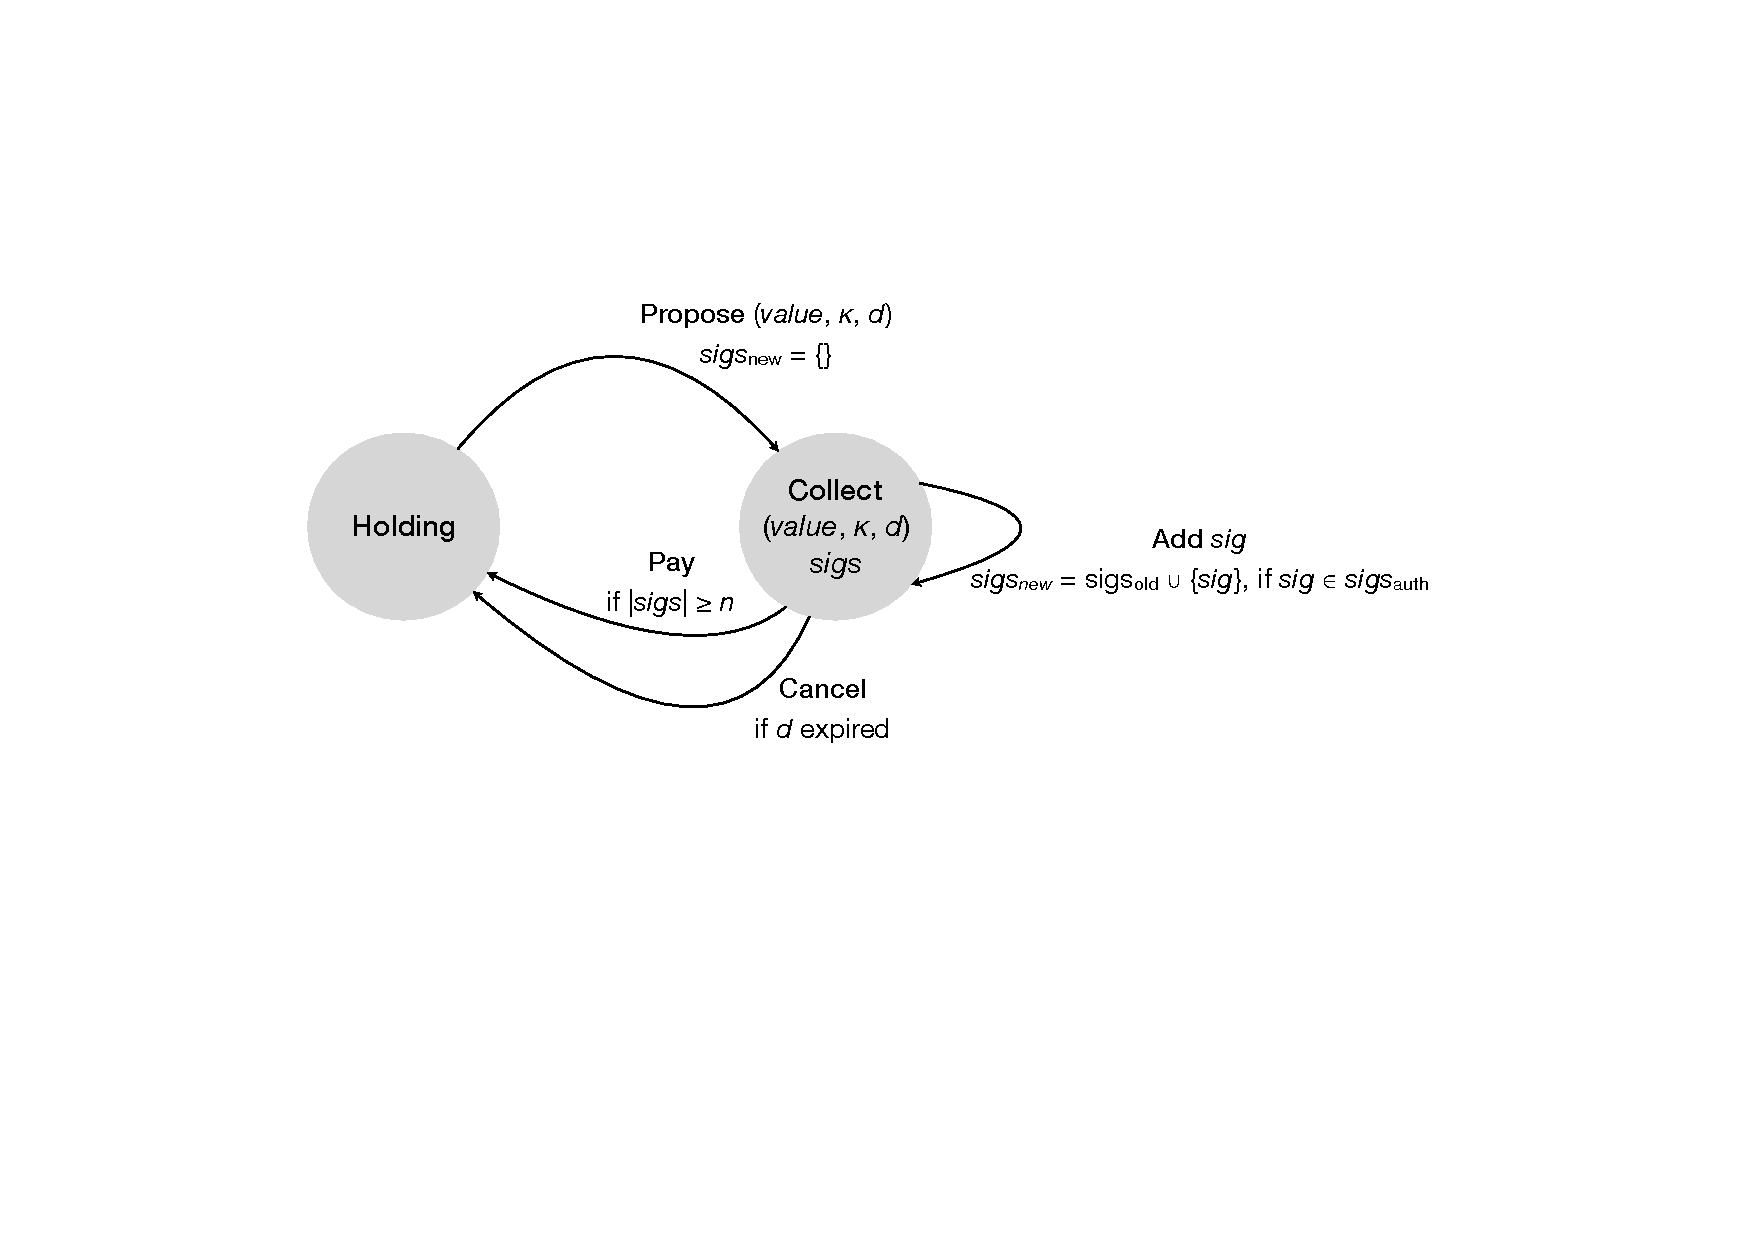
\includegraphics[width=\textwidth]{EUTxO_MultiSig_States.pdf}
  \caption{Transition diagram for the multi-signature state machine; edges labelled with input from redeemer and transition constraints.}
  \label{fig:multisig-machine}
\end{figure}
%
As a simple example of a state machine contract consider an $n$--of--$m$
multi-signature contract. Specifically, we have a given amount
$\val_\msc$ of some cryptocurrency and we require the approval of at
least $n$ out of an a priori fixed set of $m \geq n$ owners to spend
$\val_\msc$. With plain \UTXO{} (e.g., on Bitcoin), a multi-signature
scheme requires out-of-band (off-chain) communication to collect all
$n$ signatures to spend $\val_\msc$. On Ethereum, and also in the
\EUTXO{} model, we can collect the signatures on-chain, without any
out-of-band communication. To do so, we use a state machine operating
according to the transition diagram in
Figure~\ref{fig:multisig-machine}, where we assume that the threshold
$n$ and authorised signatures $\sigs_\auth$ with \(|\sigs_\auth| = m\)
are baked into the contract code.

In its implementation in the \EUTXO{} model, we use a validator
function $\nu_\msc$ accompanied by the datum $\delta_\msc$ to lock
$\val_\msc$. The datum $\delta_\msc$ stores the machine state,
which is of the form \(\Holding\) when only holding the locked value
or \(\Collecting{(\val, \kappa, d)}{\sigs}\) when collecting
signatures $\sigs$ for a payment of $\val$ to $\kappa$ by the deadline
$d$. The initial output for the contract is \((\nu_\msc, \val_\msc,
\Holding)\).

The validator $\nu_\msc$ implements the state transition diagram from
Figure~\ref{fig:multisig-machine} by using the redeemer of the spending input to determine the transition that needs to be taken. That redeemer (state machine input) can take four forms: 
\begin{inparaenum}[(1)]
\item \(\Propose{\val, \kappa, d}\) to propose a payment of $\val$ to $\kappa$
  by the deadline $d$, 
\item \(\Add{\sig}\) to add a signature $\sig$ to a payment, 
\item $\Cancel$ to cancel a proposal after its deadline expired, and 
\item $\Pay$ to make a payment once all required signatures have been collected. 
\end{inparaenum}
It then validates that the spending transaction $\mi{tx}$ is a valid
representation of the newly reached machine state. This implies that
$\mi{tx}$ needs to keep $\val_\msc$ locked by $\nu_\msc$ and that the
state in the datum $\delta^{\prime}_\msc$ needs to be the successor state
of $\delta_\msc$ according to the transition diagram.

The increased expressiveness of the \EUTXO{} model goes far beyond
simple contracts such as this on-chain multi-signature contract. For
example, the complete functionality of the Marlowe domain-specific
language for financial contracts~\cite{marlowe} has been successfully
implemented as a state machine on the \EUTXO{} model.
